%%%%%%%%%%%%%%%%%%%%
%% PSCF program
%% ~PSCFdemo.Rnw~
%% $Rev$
%% Sept. 2009
%% Satoshi Takahama (stakahama@ucsd.edu)
%%%%%%%%%%%%%%%%%%%%

\documentclass{article}
\usepackage{texmf/Sweave}

\usepackage[usenames]{color}
\definecolor{darkred}{rgb}{0.545,0,0}
\definecolor{midnightblue}{rgb}{0.098,0.098,0.439}
\DefineVerbatimEnvironment{Sinput}{Verbatim}{fontshape=sl,
formatcom=\color{midnightblue}}
\DefineVerbatimEnvironment{Soutput}{Verbatim}{formatcom=\color{darkred}}
\DefineVerbatimEnvironment{Scode}{Verbatim}{fontshape=sl,
formatcom=\color{blue}}
\fvset{listparameters={\setlength{\topsep}{2pt}}} 
\renewenvironment{Schunk}{\vspace{\topsep}}{\vspace{\topsep}} 
%%\newcommand{\minip}[2]{\begin{minipage}{#1}#2\end{minipage}}
\usepackage{fullpage}
\parindent 0in
\title{PSCF demo}
\date{}
\setkeys{Gin}{width=1.0\textwidth}
\begin{document}
\maketitle
\hrulefill
\tableofcontents
\hrulefill

\section{Preliminaries}

From this point it will be assumed that you have generated trajectory
files with HYSPLIT (following the instructions in Readme.pdf) and
combine them into a \verb@coords.rda@ file. The example
\verb@coords.rda@ file used here was generated for the VOCALS-REx campaign.\\

First, load libraries and functions. Be sure that you have the R
packges \verb@chron@, \verb@fields@, \verb@maps@, \verb@mapproj@, and
\verb@akima@ installed - this can be done very easily. For example,
while connected to the internet, type at the R prompt:

\begin{Schunk}
\begin{Sinput}
> install.packages("chron", repos = "http://cran.r-project.org")
\end{Sinput}
\end{Schunk}

After all libraries have been installed, Begin the program:
\begin{Schunk}
\begin{Sinput}
> invisible(capture.output({
+     library(chron)
+     library(fields)
+     library(maps)
+     library(mapproj)
+     library(akima)
+ }))
> mapf.env <- (if (all(regexpr("mapfunctions", search()) < 0)) attach(NULL, 
+     2, name = "mapfunctions") else pos.to.env(grep("mapfunctions", 
+     search())))
> sys.source("functions/pscf_functions.r", mapf.env)
> source("functions/classdef.r")
> options(stringsAsFactors = FALSE)
\end{Sinput}
\end{Schunk}

Functions are located in a folder called \verb@functions/@, in
\verb@functions.r@. Also located in the same folder is a file called
\verb@classdef.r@, which contains definitions for object classes used here.\\

\smallskip
User inputs - tell us where your files are:

\begin{Schunk}
\begin{Sinput}
> coordsfile <- "outputs/coords_vocals.rda"
> groupfile <- "userinputs/groupfile-example_alcf.txt"
\end{Sinput}
\end{Schunk}

Your group file should look like this:

\begin{Schunk}
\begin{Sinput}
> head(read.delim(groupfile, row.names = 1))
\end{Sinput}
\begin{Soutput}
                   Start               End Group
VX0021 10/21/08 12:03:00 10/21/08 17:32:00   low
VX0022 10/21/08 23:33:00 10/22/08 10:30:00   low
VX0024 10/22/08 11:40:00 10/22/08 21:54:00  high
VX0025 10/22/08 23:51:00 10/23/08 11:16:00  high
VX0026 10/23/08 12:28:00 10/24/08 11:09:00  high
VX0030 10/24/08 12:17:00 10/24/08 23:30:00  high
\end{Soutput}
\end{Schunk}

\section{Three main objects:  trajectories, map, and grid}

\subsection{Trajectories}

Read trajectories; shorten to 3 days (optional):

\begin{Schunk}
\begin{Sinput}
> trajectories <- readtrajectories(coordsfile)
> trajectories <- shorten(trajectories, ndays = 3)
\end{Sinput}
\end{Schunk}

Randomly sample 1/2 of trajectories for this example (remove this line
for production run).

\begin{Schunk}
\begin{Sinput}
> trajectories <- random(trajectories, fraction = 0.5)
\end{Sinput}
\end{Schunk}

\subsection{Map}

Define map [longitude (xlim) and latitude (ylim) arguments are
optional).

\begin{Schunk}
\begin{Sinput}
> mp <- definemap("world", xlim = c(-110, -50), ylim = c(-60, 5))
\end{Sinput}
\end{Schunk}

If map database is \verb~"world2"~, the longitudes have to be transformed (otherwise, leave unchanged). 
\begin{Schunk}
\begin{Sinput}
> trajectories <- transform(trajectories, mp)
\end{Sinput}
\end{Schunk}


\subsection{Grid}
Define grid. The following line will divide the box containing trajectory
endpoints (both latittude and longitude) into 40 even-sized boxes.
\begin{Schunk}
\begin{Sinput}
> xygrid <- definegrid(traj = trajectories, len = 40)
\end{Sinput}
\end{Schunk}

Alternatively, you can specify the grid coordinates directly (not run in this example).
\begin{Schunk}
\begin{Sinput}
> xygrid <- definegrid(longrid = seq(-95, 50, 5), latgrid = seq(35, 
+     93, 3))
\end{Sinput}
\end{Schunk}

\section{Evaluate map and grid}


Look at the map boundaries and spacing of grid points overlayed on
map; redefine if necessary. 

\begin{Schunk}
\begin{Sinput}
> par(mfrow = c(1, 2), mar = rep(1, 4))
> showmap(mp, gridlines = TRUE)
> showmap(mp, xygrid)
\end{Sinput}
\end{Schunk}
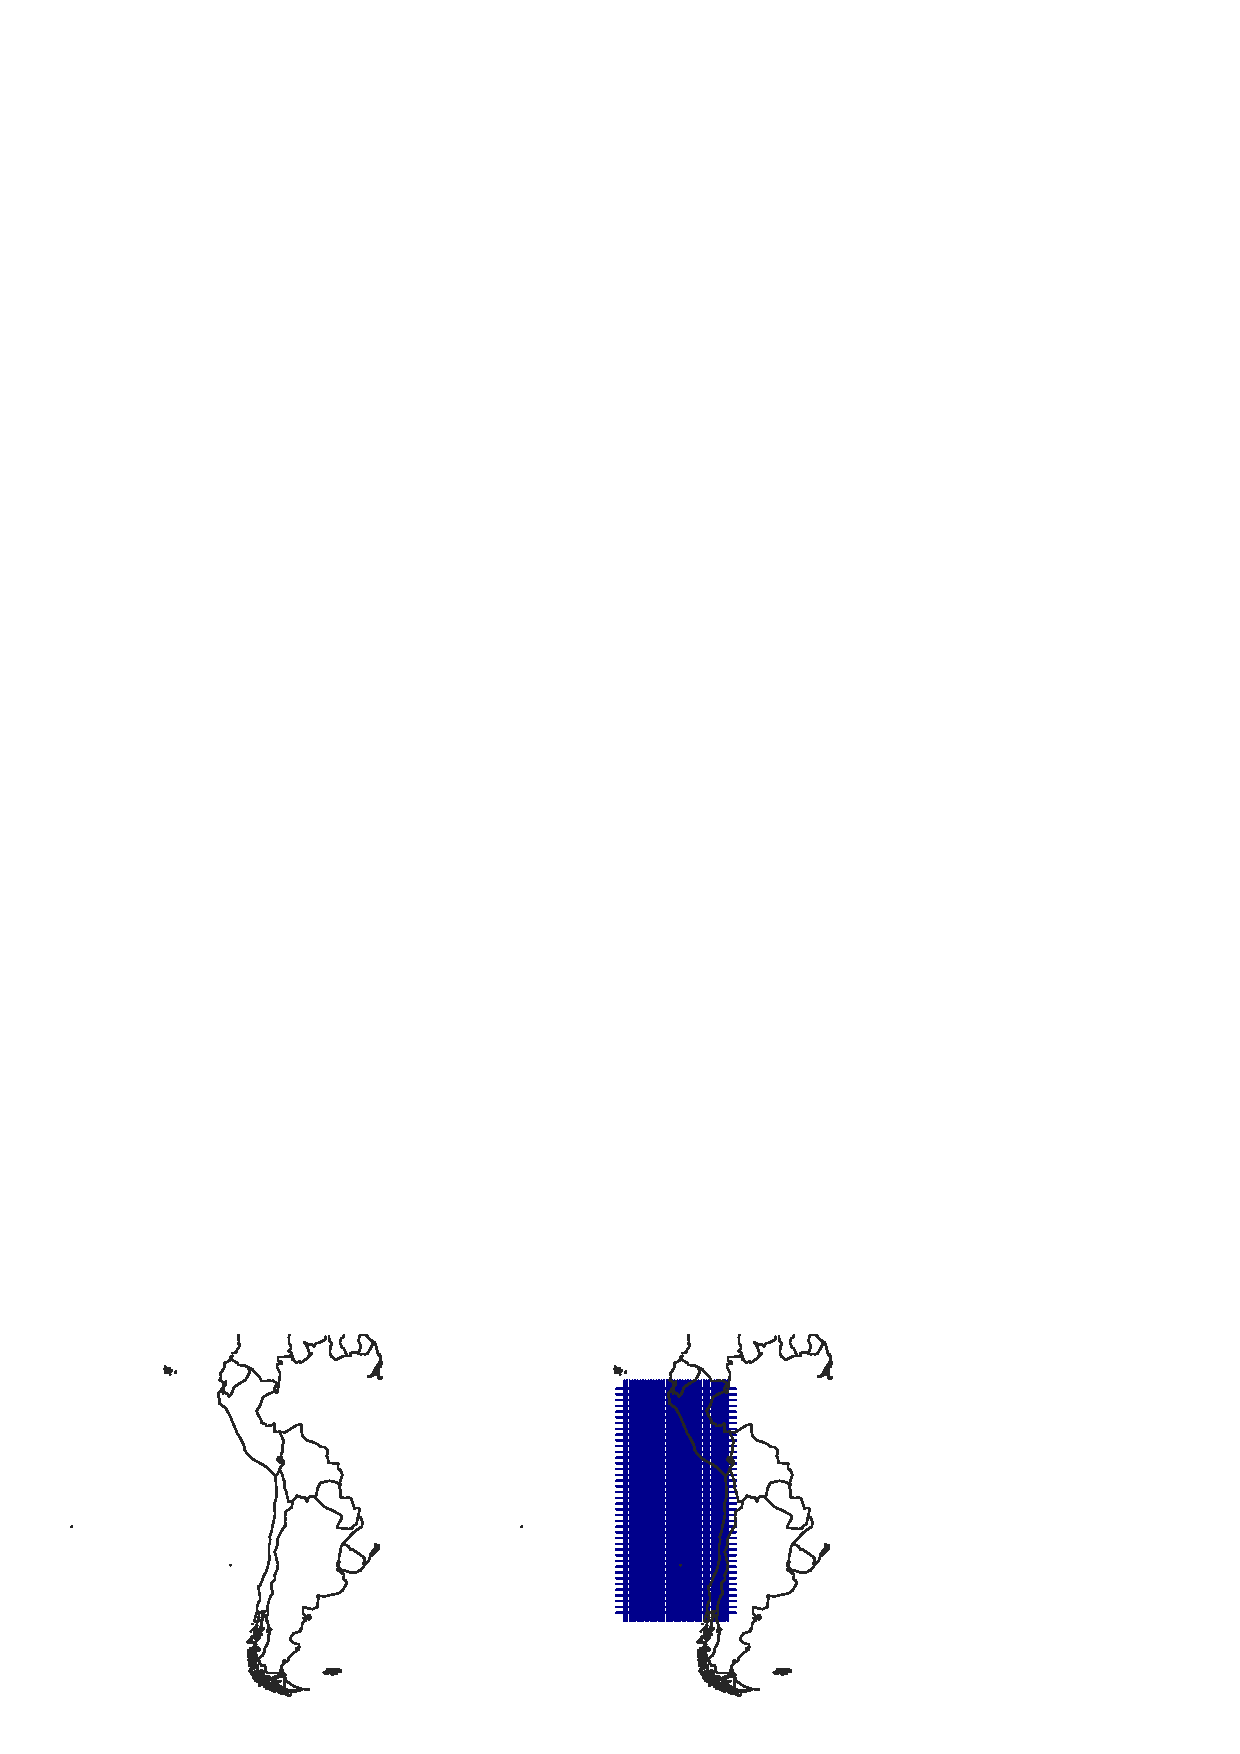
\includegraphics{figures/fig-012}

\section{Prepare the trajectories}


Overlay trajectories on the grid [the last argument can be either
\verb@identity@ to count number of trajectory points (default), or
\verb@unique@ to count unique trajectories over each grid cell]:

\begin{Schunk}
\begin{Sinput}
> trajectories <- overlay(trajectories, xygrid, identity)
\end{Sinput}
\end{Schunk}

(See \verb@reports/identity-unique/summary.pdf@ for comparison between
the two options.)\\

Read in group file and prepare trajectory object for visualization; attach data
to 'trajectories' object. If new groups are desired, rerun from this point on
(do not have to reload trajectories).

\begin{Schunk}
\begin{Sinput}
> groups(trajectories) <- readgroups(groupfile)
> trajectories <- prepareforvis(trajectories, xygrid)
\end{Sinput}
\end{Schunk}

\section{Plotting trajectories}

\subsection{Examples - VOCALS}
Show all trajectories (as 'spaghetti' and 'density'):

\begin{Schunk}
\begin{Sinput}
> par(mfrow = c(1, 2), mar = rep(1, 4))
> showmap(mp, trajectories, type = "spaghetti", groupindex = 0, 
+     gridlines = TRUE)
> showmap(mp, trajectories, type = "density", groupindex = 0, gridlines = TRUE)
\end{Sinput}
\end{Schunk}
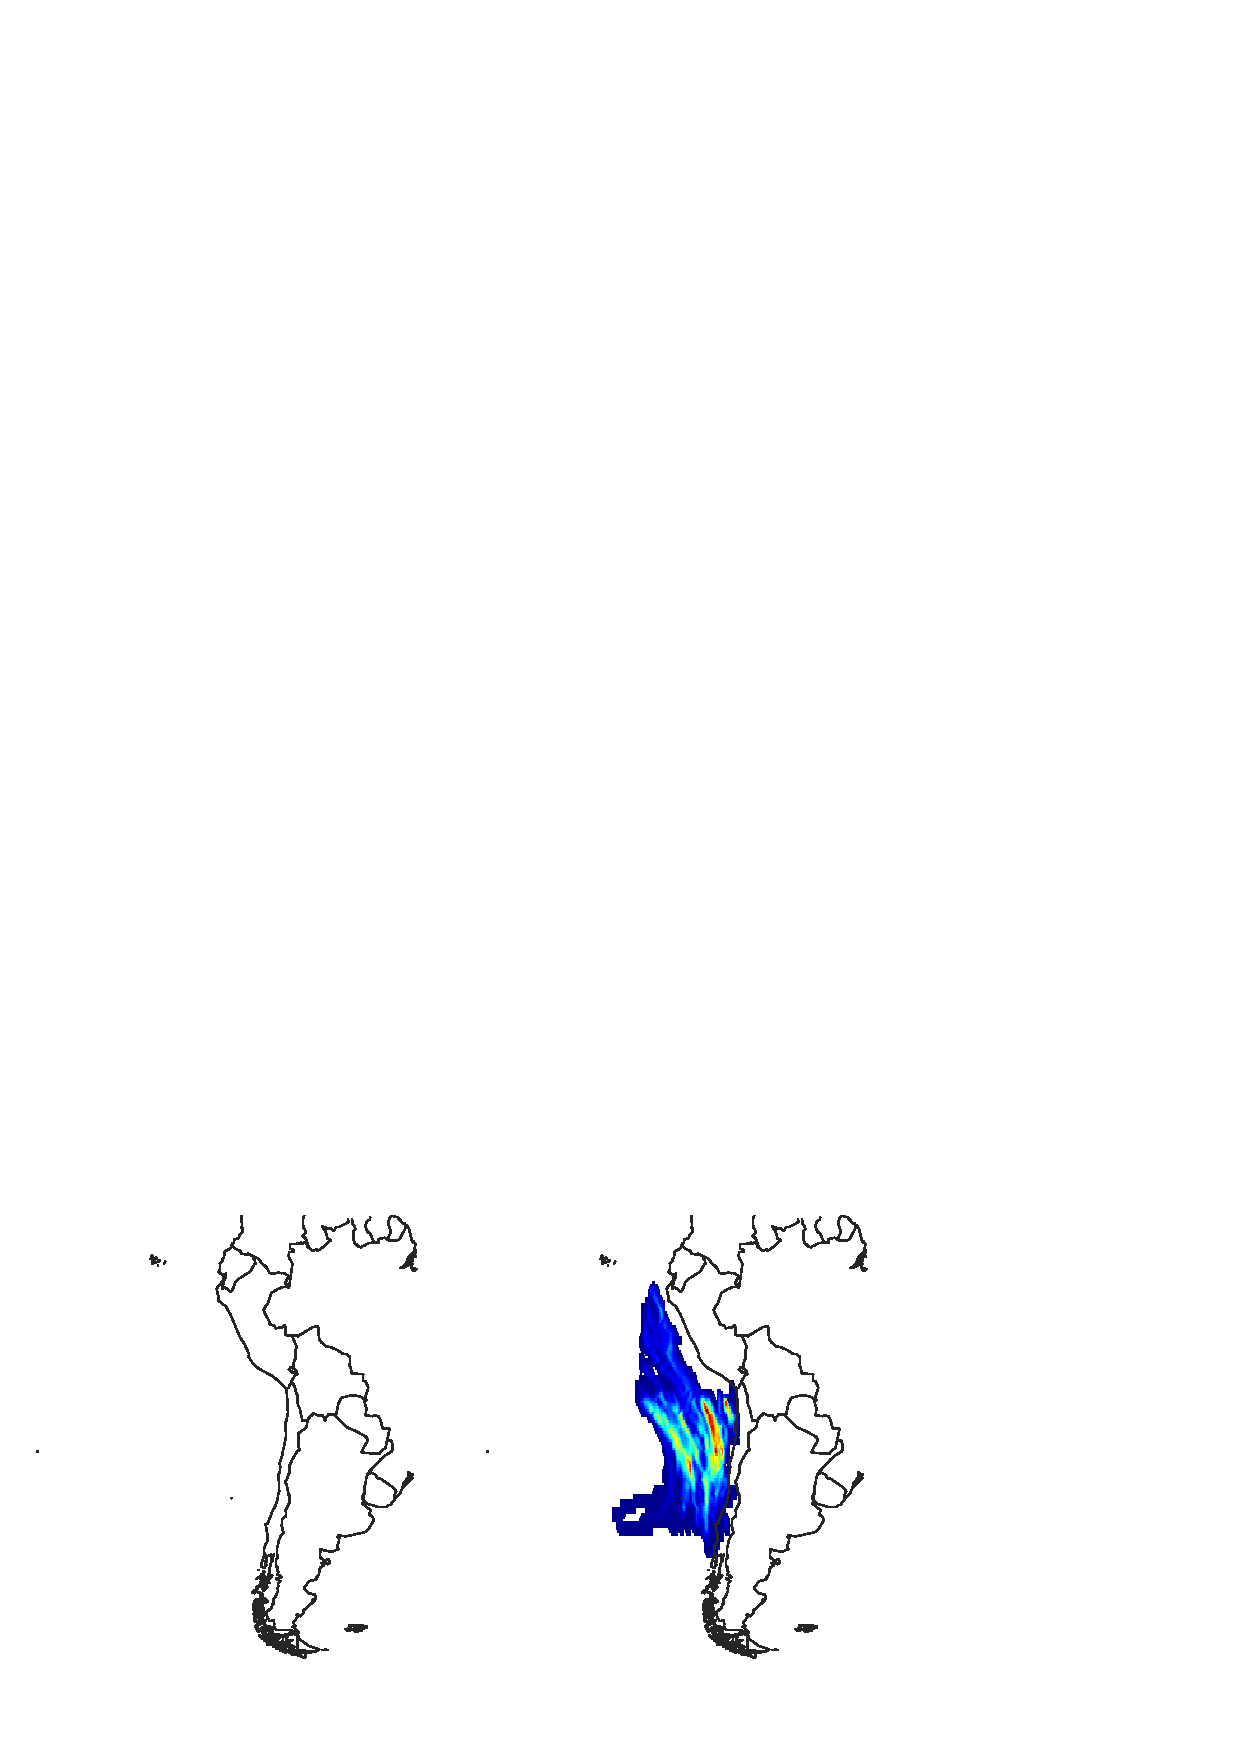
\includegraphics{figures/fig-015}

Next, visualize number of trajectories/ points per cell.

\begin{Schunk}
\begin{Sinput}
> par(mfrow = c(1, 1), mar = c(4.5, 4.5, 1.5, 1.5), mgp = c(2.5, 
+     1, 0), pty = "s")
> cumuldensp(trajectories)
\end{Sinput}
\end{Schunk}
\includegraphics{figures/fig-016}

We will only include grid cells for which the number of
trajectories/points (count/cell) are above 10, approximately (values
$<$1 indicate cells in which weights ($\to$ fraction of hour) were
$<$1), so we pass the argument \verb@threshold=0.4@ to the
\verb@showmap()@ function. The PSCF plot is created with the following
code. Export with graphics desired device (e.g., \verb@pdf()@,
\verb@png()@).

\begin{Schunk}
\begin{Sinput}
> ngr <- length(groups(trajectories))
> layout(matrix(1:(ngr + 1), nrow = 1), width = c(rep(5, ngr), 
+     1))
> par(mar = c(1, 1, 1.5, 1), mgp = c(1, 1, 0), lend = 3, pty = "s")
> for (i in 1:ngr) {
+     showmap(mp, trajectories, threshold = 0.4, type = "pscf", 
+         groupindex = i, gridlines = TRUE)
+     title(main = grpname(trajectories, i), cex.main = 1.2)
+ }
> addlegend(m1 = 2, m2 = 1.5, m3 = 2, m4 = 2, mgp = c(2, 0.5, 0), 
+     cex.axis = 0.6)
\end{Sinput}
\end{Schunk}
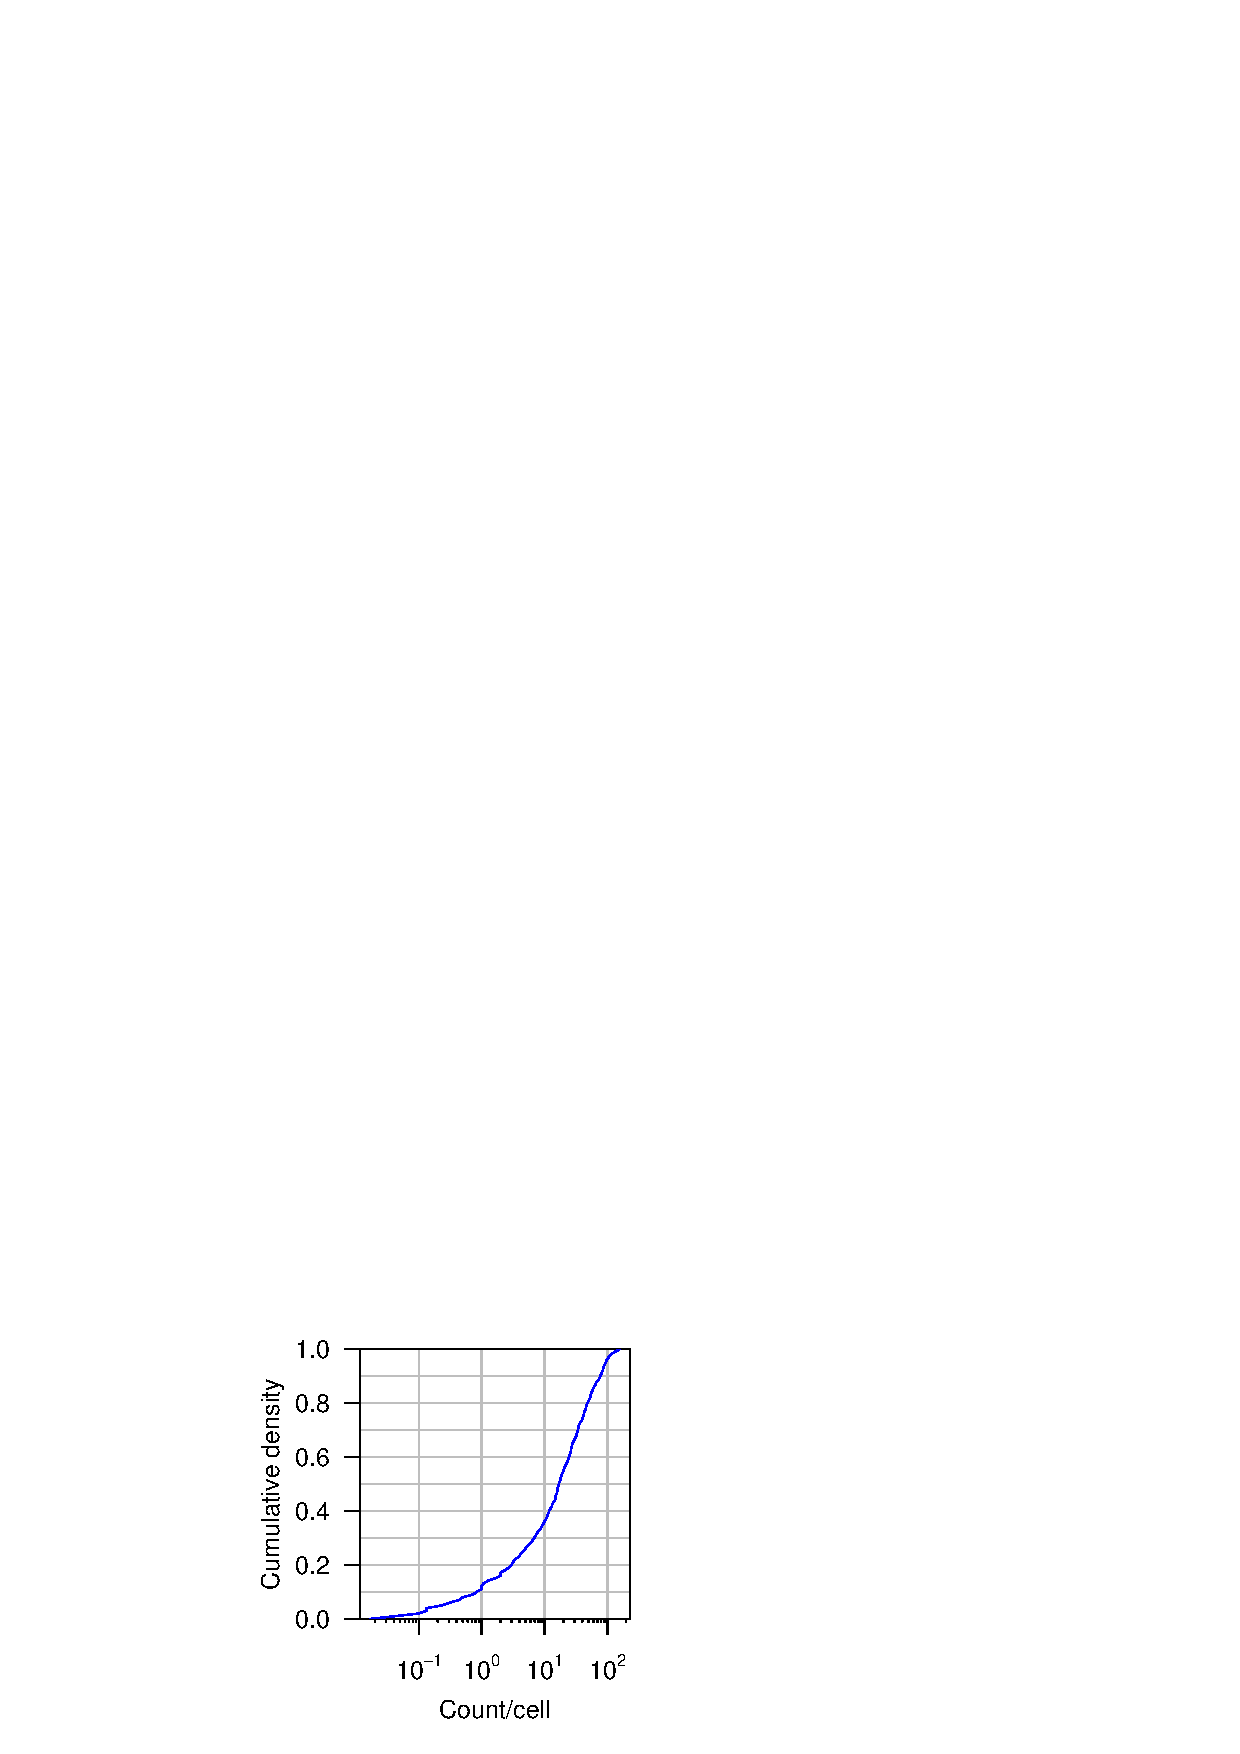
\includegraphics{figures/fig-017}

\subsection{Additional examples: shiptracks, other projections (not run)}


We can also add ship tracks. Calculate it from the originating point
for each of the back trajectories:

\begin{Schunk}
\begin{Sinput}
> shiptrack <- lapply(colnames(coords(trajectories))[2:1], function(x, 
+     y) sapply(y[, x], `[`, 1), coords(trajectories))
\end{Sinput}
\end{Schunk}

Plot ship tracks. For an orthographic projection, we don't need x- and
y-limits. To get rid of them, redefine the map without passing values
to \verb@xlim@ and \verb@ylim@ parameters.

\begin{Schunk}
\begin{Sinput}
> mp <- definemap("world")
\end{Sinput}
\end{Schunk}

Make the plot:

\begin{Schunk}
\begin{Sinput}
> showmap(mp, shiptrack = shiptrack, projection = "orthographic", 
+     orientation = c(90, 0, -12.5))
\end{Sinput}
\end{Schunk}

Map in stereographic projection:

\begin{Schunk}
\begin{Sinput}
> par(mfrow = c(1, 2), mar = rep(1, 4))
> showmap(mp, gridlines = TRUE)
> showmap(mp, xygrid)
\end{Sinput}
\end{Schunk}

PSCF map with shiptracks in stereographic projection:

\begin{Schunk}
\begin{Sinput}
> ngr <- length(groups(trajectories))
> layout(matrix(1:(ngr + 1), , nrow = 1), width = c(rep(5, ngr), 
+     1))
> par(mar = c(1, 1, 1.5, 1), mgp = c(1, 1, 0), lend = 3, pty = "s")
> for (i in 1:ngr) {
+     showmap(mp, trajectories, shiptrack = shiptrack, type = "pscf", 
+         gridlines = TRUE, groupindex = i, projection = "stereographic")
+     title(main = grpname(trajectories, i), cex.main = 1.2)
+ }
> addlegend(m1 = 2, m2 = 1.5, m3 = 2, m4 = 2, mgp = c(2, 0.5, 0), 
+     cex.axis = 0.6)
\end{Sinput}
\end{Schunk}

\subsection{The showmap() function}


Summary of arguments to \verb@showmap@:

\begin{center}
  \begin{tabular}{ll}
    Argument & Possible values \\
    \hline
    \verb@mobj@ & 'Map' object (*required*) \\
    \verb@obj1@ & 'XYGrid' or 'Traj' object \\
    \verb@type@ & 'diagnose', 'spaghetti', 'density', or 'pscf' (character)\\
    \verb@gridlines@ & TRUE or FALSE (logical) \\
    \verb@groupindex@ & 1,2,...n or 0 for 'spaghetti' or 'density'
    (integer)\\
    \verb@shiptrack@ & list with longitude and latitude components
    (list)\\
    \verb@threshold@ & \begin{minipage}{0.5\textwidth}exclude grid cells
      containing less than \verb@threshold@ quantile (percentile /100)
      of trajectory counts.\end{minipage}\\ 
    \verb@...@ & projection and parameters to be pased to \verb@mapproject@ \\
  \end{tabular}
\end{center}

The 'Map' object is the only required argument. Not specifying a value
for \verb@projection@ will give you a rectangular projection.\\

\verb@showmap()@ is intended to be an exploratory tool. Edit function
\verb@mpj()@ in \verb@functions/classdefs.r@ if further customizations
are desired.

\section{Misc.}

\subsection{Image resolution}

Increasing/decreasing image resolution using the \verb@ninterp@
argument to \verb@showmap()@ - compare with left PSCF figure - 'high'
case. In this case I decreased the resolution to constrast the visual
difference in appearance.
\begin{Schunk}
\begin{Sinput}
> showmap(mp, trajectories, type = "pscf", gridlines = TRUE, groupindex = 1, 
+     ninterp = 30)
> title(main = grpname(trajectories, 1), cex.main = 1.2)
\end{Sinput}
\end{Schunk}
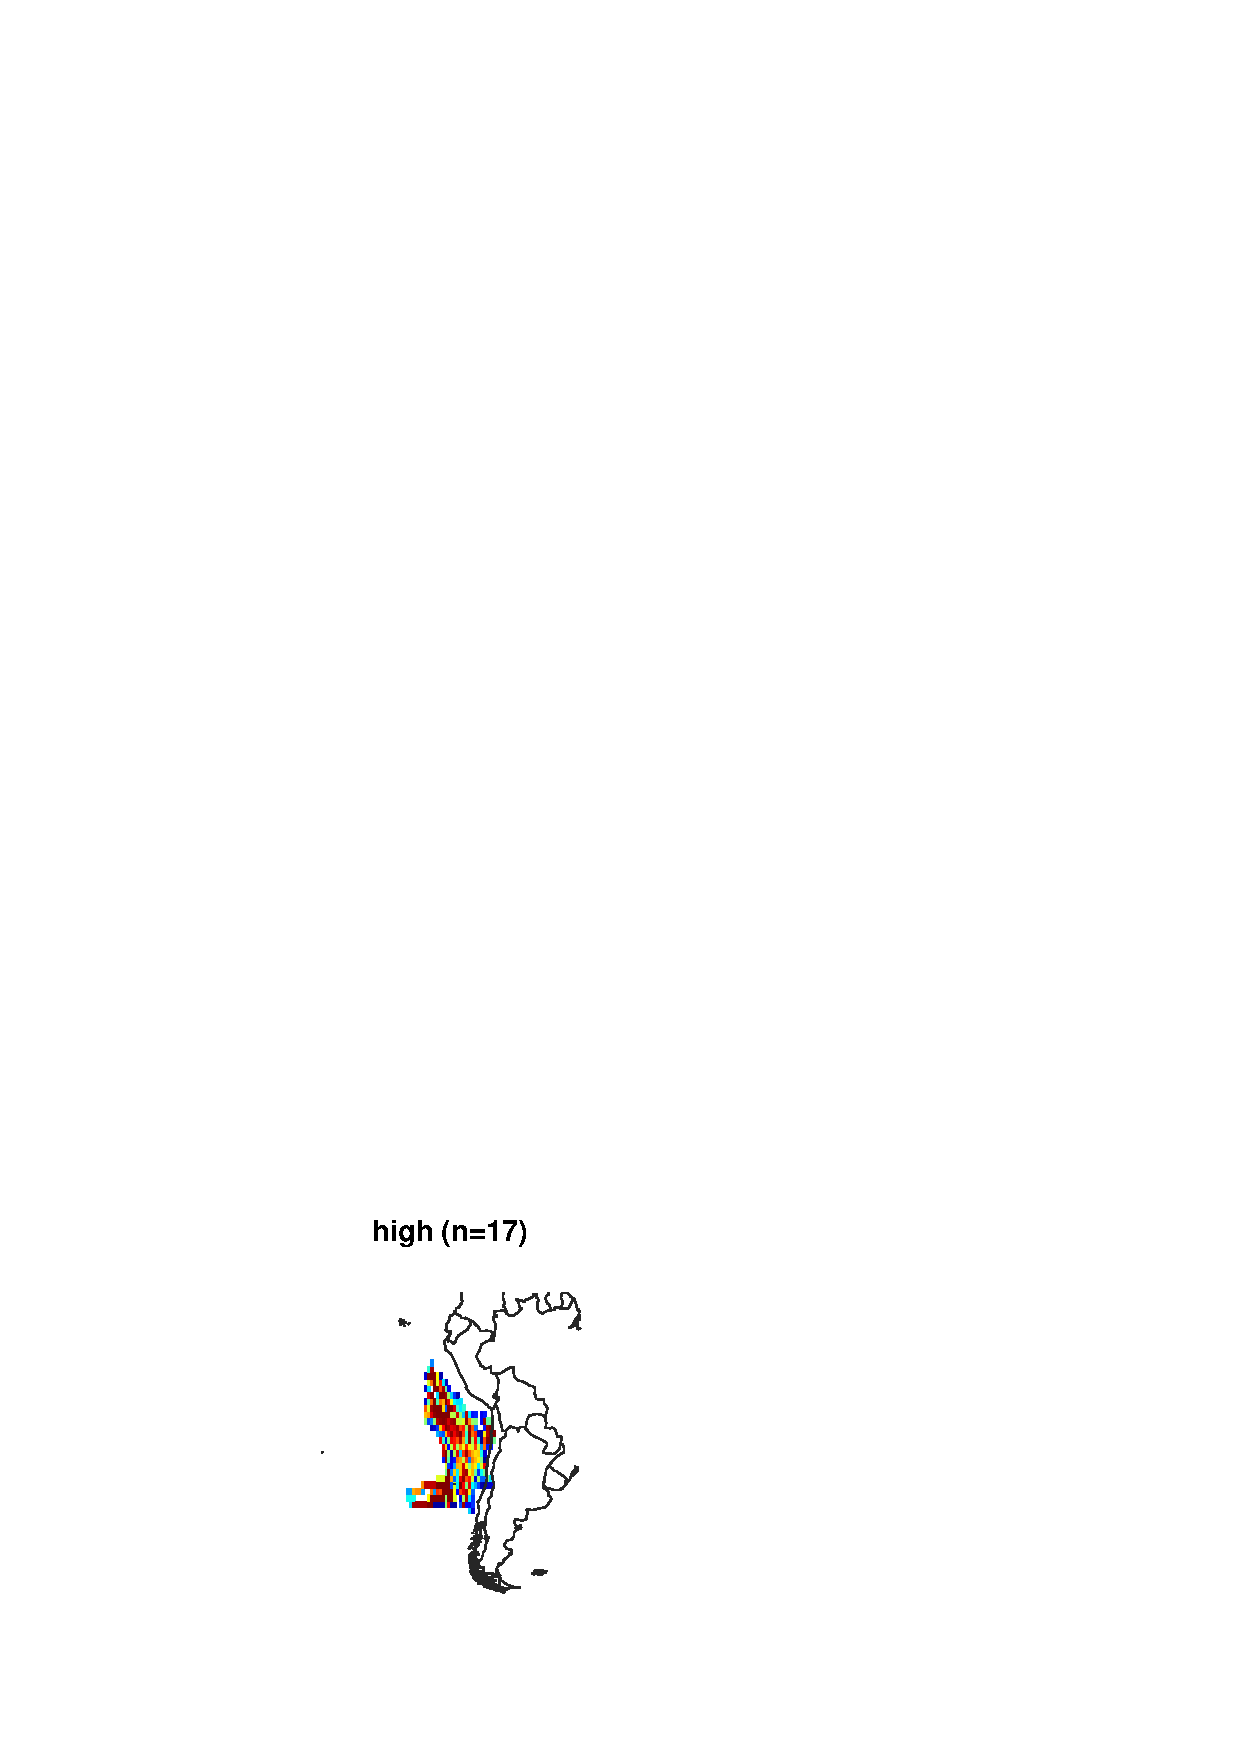
\includegraphics{figures/fig-023}

\subsection{Data extraction for export/ customization}

Use \verb@extract()@ on object \verb@trajectories@. (You can also pass
a \verb@threshold@ argument to \verb@extract()@). Note: matrix
resolution is defined by \verb@xygrid@ using \verb@definegrid()@;
\verb@ninterp@ is only used for controlling resolution for
visualization using \verb@showmap()@.
\begin{Schunk}
\begin{Sinput}
> output <- extract(trajectories, type = "pscf", groupindex = 1, 
+     threshold = 0.4)
\end{Sinput}
\end{Schunk}

You can export the data using \verb@write()@:
\begin{Schunk}
\begin{Sinput}
> write(output$x, file = "xvalues.txt", ncol = 1)
> write(output$y, file = "yvalues.txt", ncol = 1)
> write(t(output$z), file = "zvalues.txt", ncol = ncol(output$z))
\end{Sinput}
\end{Schunk}

Or plot it in R using \verb@image()@ (which is called internally by
\verb@showmap()@). 
\begin{Schunk}
\begin{Sinput}
> image(output, col = grey.colors(64), asp = 1)
\end{Sinput}
\end{Schunk}
\includegraphics{figures/fig-026}

\end{document}
